\documentclass[20pt]{article} 

\setlength{\oddsidemargin}{0.0in}
\setlength{\evensidemargin}{0.0in}
\setlength{\topmargin}{0.0in}
\setlength{\headheight}{0in}
\setlength{\headsep}{0in}
\setlength{\textwidth}{6.5in}
\setlength{\textheight}{9.0in}
\setlength{\parindent}{0.2in}
\setlength{\parskip}{0.1in}

\usepackage{times}
\usepackage{fancyvrb}
\usepackage{relsize}
\usepackage{color}

\usepackage{graphicx}

\usepackage{amsmath}

\usepackage{hyperref}


\begin{document} 

\definecolor{offwhite}{gray}{0.92}
\definecolor{GreenYellow}{cmyk}{0.15,0,0.69,0}
\definecolor{Tan}{cmyk}{0.14,0.42,0.56,0}
\definecolor{GrayLight}{cmyk}{0,0,0,0.15}
\definecolor{RawSienna}{cmyk}{0,0.72,1,0.45}
\definecolor{TealBlue}{cmyk}{0.86,0,0.34,0.02}
\definecolor{Aquamarine}{cmyk}{0.82,0,0.30,0}
\definecolor{BlueGreen}{cmyk}{0.85,0,0.33,0}
\definecolor{Emerald}{cmyk}{1,0,0.50,0}
\definecolor{JungleGreen}{cmyk}{0.99,0,0.52,0}
\definecolor{SeaGreen}{cmyk}{0.69,0,0.50,0}
\definecolor{Green}{cmyk}{1,0,1,0}
\definecolor{ForestGreen}{cmyk}{0.91,0,0.88,0.12}
\definecolor{PineGreen}{cmyk}{0.92,0,0.59,0.25}
\definecolor{LimeGreen}{cmyk}{0.50,0,1,0}
\definecolor{YellowGreen}{cmyk}{0.44,0,0.74,0}
\definecolor{SpringGreen}{cmyk}{0.26,0,0.76,0}
\definecolor{OliveGreen}{cmyk}{0.64,0,0.95,0.40}

\definecolor{Peach}{cmyk}{0,0.50,0.70,0}
\definecolor{Melon}{cmyk}{0,0.46,0.50,0}
\definecolor{YellowOrange}{cmyk}{0,0.42,1,0}
\definecolor{Orange}{cmyk}{0,0.61,0.87,0}
\definecolor{BurntOrange}{cmyk}{0,0.51,1,0}
\definecolor{Bittersweet}{cmyk}{0,0.75,1,0.24}
\definecolor{RedOrange}{cmyk}{0,0.77,0.87,0}
\definecolor{Mahogany}{cmyk}{0,0.85,0.87,0.35}
\definecolor{Maroon}{cmyk}{0,0.8,0.68,0.32}
\definecolor{BrickRed}{cmyk}{0,0.89,0.94,0.28}

\definecolor{CadetBlue}{cmyk}{0.62,0.57,0.23,0} % PANTONE (534+535)
\definecolor{CornflowerBlue}{cmyk}{0.65,0.13,0,0} % PANTONE 292
\definecolor{MidnightBlue}{cmyk}{0.98,0.13,0,0.43} % PANTONE 302
\definecolor{NavyBlue}{cmyk}{0.94,0.54,0,0} % PANTONE 293
\definecolor{RoyalBlue}{cmyk}{1.,0.50,0,0} % No PANTONE match
\definecolor{Blue}{cmyk}{1.,1.,0,0} % PANTONE BLUE-072
\definecolor{Cerulean}{cmyk}{0.94,0.11,0,0} % PANTONE 3005
\definecolor{Cyan}{cmyk}{1.,0,0,0} % PANTONE PROCESS-CYAN
\definecolor{ProcessBlue}{cmyk}{0.96,0,0,0} % PANTONE PROCESS-BLUE
\definecolor{SkyBlue}{cmyk}{0.62,0,0.12,0} % PANTONE 2985
\definecolor{Turquoise}{cmyk}{0.85,0,0.20,0} % PANTONE (312+313)
\definecolor{RubineRed}{cmyk}{0,1.,0.13,0} % PANTONE RUBINE-RED
\definecolor{WildStrawberry}{cmyk}{0,0.96,0.39,0} % PANTONE 206
\definecolor{Salmon}{cmyk}{0,0.53,0.38,0} % PANTONE 183
\definecolor{CarnationPink}{cmyk}{0,0.63,0,0} % PANTONE 218
\definecolor{Magenta}{cmyk}{0,1.,0,0} % PANTONE PROCESS-MAGENTA
\definecolor{VioletRed}{cmyk}{0,0.81,0,0} % PANTONE 219
\definecolor{Rhodamine}{cmyk}{0,0.82,0,0} % PANTONE RHODAMINE-RED
\definecolor{Mulberry}{cmyk}{0.34,0.90,0,0.02} % PANTONE 241
\definecolor{RedViolet}{cmyk}{0.07,0.90,0,0.34} % PANTONE 234
\definecolor{Fuchsia}{cmyk}{0.47,0.91,0,0.08} % PANTONE 248
\definecolor{Lavender}{cmyk}{0,0.48,0,0} % PANTONE 223
\definecolor{Thistle}{cmyk}{0.12,0.59,0,0} % PANTONE 245
\definecolor{Orchid}{cmyk}{0.32,0.64,0,0} % PANTONE 252
\definecolor{DarkOrchid}{cmyk}{0.40,0.80,0.20,0} %  No PANTONE match
\definecolor{Purple}{cmyk}{0.45,0.86,0,0} % PANTONE PURPLE
\definecolor{Plum}{cmyk}{0.50,1.,0,0} % PANTONE 518
\definecolor{Violet}{cmyk}{0.79,0.88,0,0} % PANTONE VIOLET
\definecolor{RoyalPurple}{cmyk}{0.75,0.90,0,0} % PANTONE 267
\definecolor{BlueViolet}{cmyk}{0.86,0.91,0,0.04} % PANTONE 2755

\definecolor{Sepia}{cmyk}{0,0.83,1,0.70}
\definecolor{save1}{cmyk}{0.19,0.0,0.3,0.0}
\definecolor{save2}{cmyk}{0.09,0.0,0.3,0.0}
\definecolor{save3}{cmyk}{0.03,0.0,0.2,0.0}
\definecolor{save4}{cmyk}{0.03,0.1,0.2,0.0}
\definecolor{save5}{cmyk}{0.13,0.1,0.1,0.0}
\definecolor{save6}{cmyk}{0.0,0.0,0.3,0.05}
\definecolor{myblue}{rgb}{0.0,0.5,0.1}
\definecolor{save7w}{cmyk}{0.8,0.0,0.8,0.25}
\definecolor{x}{cmyk}{0.0,0.0,0.8,0.0}

% \pagecolor{Mahogany}
% \pagecolor{BrickRed}
% \pagecolor{BurntOrange}
% \pagecolor{RedOrange}
% \pagecolor{OliveGreen}
% \pagecolor{BlueViolet}
% MidnightBlue with white lettering is cool!
\pagecolor{MidnightBlue}
\color{white}

\begin{center}
{\Huge From Algorithms to Z-Scores: 

\bigskip

Probabilistic and Statistical Modeling in Computer Science}

\bigskip

{\LARGE Norm Matloff 

\medskip

University of California, Davis}
\end{center}

\vspace{0.9in}

\begin{center}
\begin{figure}[ht]
\color{white}
   \begin{minipage}[b]{0.55\linewidth}
       \Large
       $
       \mbox{\boldmath$ f_X(t) = c e^{-0.5 (t-\mu)'\Sigma^{-1}(t-\mu)}$ } 
       $
   \end{minipage}
   \hspace{0.1in}
   \begin{minipage}[b]{0.58\linewidth}
       {\bf
       \begin{Verbatim}[fontsize=\relsize{+1}]
       library(MASS) 
       x <- mvrnorm(mu,sgm)
       \end{Verbatim}
       }
   \end{minipage}
\end{figure}
\end{center}

\vspace{-0.5in}
\centering
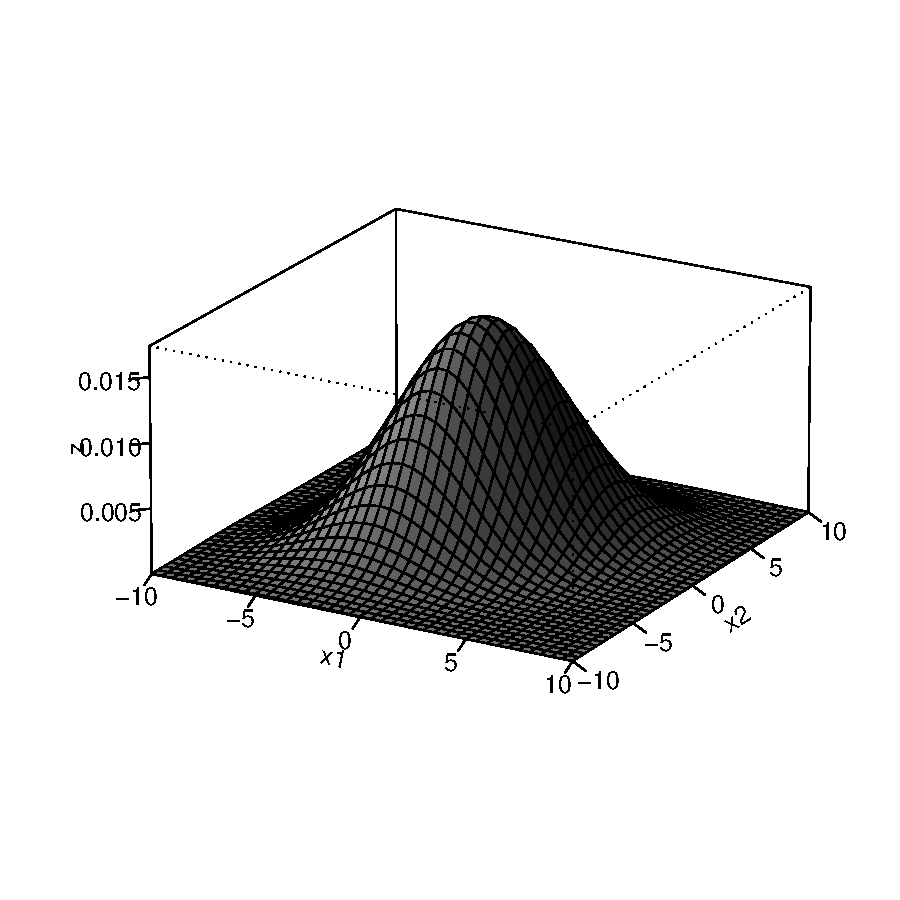
\includegraphics[width=4.8in]{Bell.pdf}

{\LARGE
{http://heather.cs.ucdavis.edu/~matloff/probstatbook.html}
}

\end{document}

